% Created by tikzDevice version 0.8.1 on 2015-06-28 00:11:20
% !TEX encoding = UTF-8 Unicode
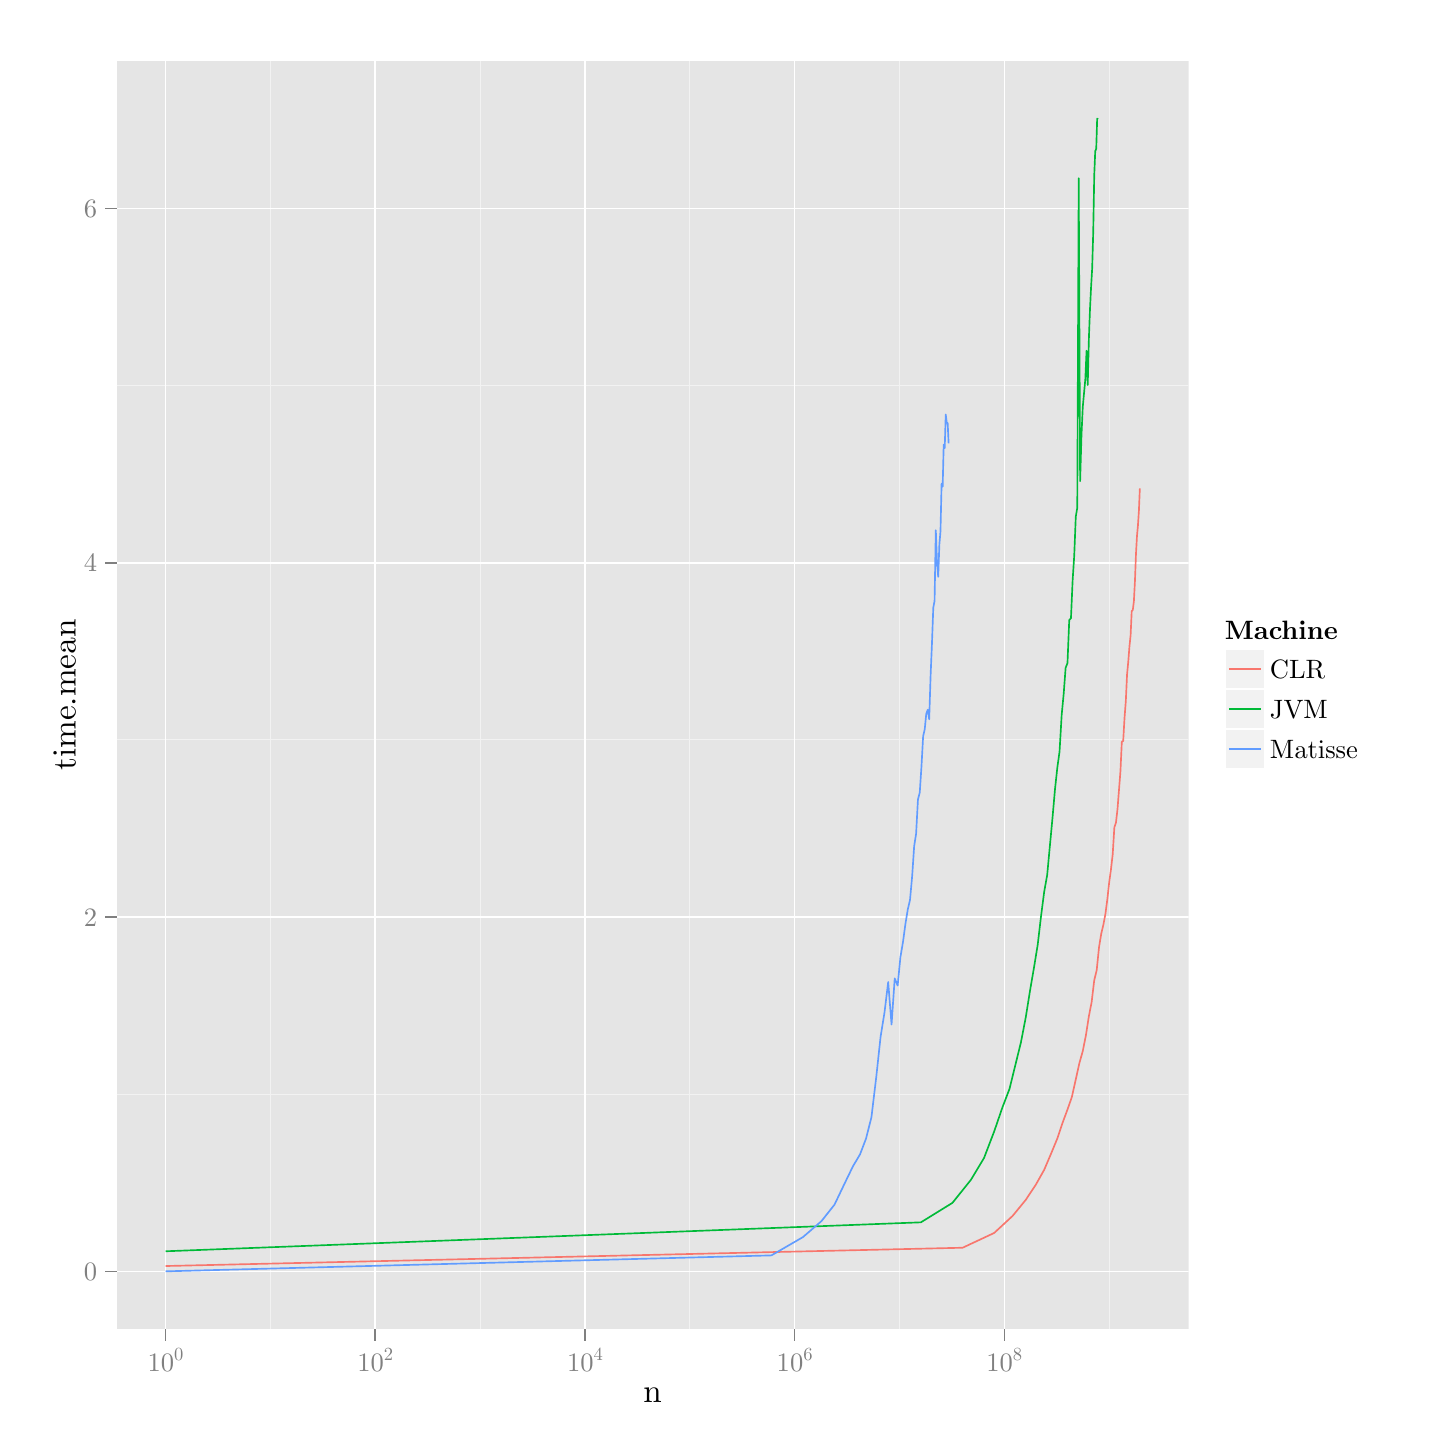
\begin{tikzpicture}[x=1pt,y=1pt]
\definecolor{fillColor}{RGB}{255,255,255}
\path[use as bounding box,fill=fillColor,fill opacity=0.00] (0,0) rectangle (505.89,505.89);
\begin{scope}
\path[clip] (  0.00,  0.00) rectangle (505.89,505.89);
\definecolor{drawColor}{RGB}{255,255,255}
\definecolor{fillColor}{RGB}{255,255,255}

\path[draw=drawColor,line width= 0.6pt,line join=round,line cap=round,fill=fillColor] (  0.00,  0.00) rectangle (505.89,505.89);
\end{scope}
\begin{scope}
\path[clip] ( 32.22, 35.66) rectangle (419.48,493.85);
\definecolor{fillColor}{gray}{0.90}

\path[fill=fillColor] ( 32.22, 35.66) rectangle (419.48,493.85);
\definecolor{drawColor}{gray}{0.95}

\path[draw=drawColor,line width= 0.3pt,line join=round] ( 32.22,120.50) --
	(419.48,120.50);

\path[draw=drawColor,line width= 0.3pt,line join=round] ( 32.22,248.53) --
	(419.48,248.53);

\path[draw=drawColor,line width= 0.3pt,line join=round] ( 32.22,376.57) --
	(419.48,376.57);

\path[draw=drawColor,line width= 0.3pt,line join=round] ( 87.71, 35.66) --
	( 87.71,493.85);

\path[draw=drawColor,line width= 0.3pt,line join=round] (163.48, 35.66) --
	(163.48,493.85);

\path[draw=drawColor,line width= 0.3pt,line join=round] (239.26, 35.66) --
	(239.26,493.85);

\path[draw=drawColor,line width= 0.3pt,line join=round] (315.03, 35.66) --
	(315.03,493.85);

\path[draw=drawColor,line width= 0.3pt,line join=round] (390.81, 35.66) --
	(390.81,493.85);
\definecolor{drawColor}{RGB}{255,255,255}

\path[draw=drawColor,line width= 0.6pt,line join=round] ( 32.22, 56.49) --
	(419.48, 56.49);

\path[draw=drawColor,line width= 0.6pt,line join=round] ( 32.22,184.52) --
	(419.48,184.52);

\path[draw=drawColor,line width= 0.6pt,line join=round] ( 32.22,312.55) --
	(419.48,312.55);

\path[draw=drawColor,line width= 0.6pt,line join=round] ( 32.22,440.58) --
	(419.48,440.58);

\path[draw=drawColor,line width= 0.6pt,line join=round] ( 49.82, 35.66) --
	( 49.82,493.85);

\path[draw=drawColor,line width= 0.6pt,line join=round] (125.60, 35.66) --
	(125.60,493.85);

\path[draw=drawColor,line width= 0.6pt,line join=round] (201.37, 35.66) --
	(201.37,493.85);

\path[draw=drawColor,line width= 0.6pt,line join=round] (277.14, 35.66) --
	(277.14,493.85);

\path[draw=drawColor,line width= 0.6pt,line join=round] (352.92, 35.66) --
	(352.92,493.85);
\definecolor{drawColor}{RGB}{248,118,109}

\path[draw=drawColor,line width= 0.6pt,line join=round] ( 49.82, 58.41) --
	(337.84, 65.02) --
	(349.25, 70.36) --
	(355.92, 76.54) --
	(360.65, 82.31) --
	(364.32, 87.85) --
	(367.32, 93.19) --
	(369.86, 99.16) --
	(372.06,104.50) --
	(373.99,110.26) --
	(375.73,114.95) --
	(377.30,119.44) --
	(378.73,125.84) --
	(380.05,131.81) --
	(381.26,136.08) --
	(382.40,141.84) --
	(383.46,148.67) --
	(384.46,153.79) --
	(385.40,161.69) --
	(386.29,165.31) --
	(387.13,173.64) --
	(387.94,178.54) --
	(388.70,181.74) --
	(389.43,185.59) --
	(390.13,190.92) --
	(390.81,197.11) --
	(391.45,201.80) --
	(392.07,207.14) --
	(392.67,216.95) --
	(393.25,218.66) --
	(393.81,223.57) --
	(394.34,230.40) --
	(394.87,237.23) --
	(395.37,247.89) --
	(395.86,248.11) --
	(396.34,256.43) --
	(396.80,262.40) --
	(397.26,272.22) --
	(397.69,276.70) --
	(398.12,282.25) --
	(398.54,286.30) --
	(398.94,295.05) --
	(399.34,295.48) --
	(399.73,298.68) --
	(400.11,305.94) --
	(400.48,315.75) --
	(400.84,322.15) --
	(401.19,325.99) --
	(401.54,331.33) --
	(401.88,339.44);
\definecolor{drawColor}{RGB}{0,186,56}

\path[draw=drawColor,line width= 0.6pt,line join=round] ( 49.82, 63.74) --
	(322.77, 74.20) --
	(334.17, 81.24) --
	(340.84, 89.56) --
	(345.58, 97.46) --
	(349.25,107.06) --
	(352.25,115.81) --
	(354.78,122.42) --
	(356.98,131.39) --
	(358.92,139.28) --
	(360.65,148.24) --
	(362.22,158.06) --
	(363.65,166.38) --
	(364.97,174.49) --
	(366.19,184.95) --
	(367.32,193.69) --
	(368.39,199.67) --
	(369.38,210.34) --
	(370.32,220.37) --
	(371.21,230.61) --
	(372.06,238.51) --
	(372.86,244.27) --
	(373.63,257.50) --
	(374.36,265.18) --
	(375.06,274.57) --
	(375.73,276.28) --
	(376.37,291.85) --
	(376.99,292.49) --
	(377.59,306.15) --
	(378.17,315.11) --
	(378.73,329.20) --
	(379.27,332.40) --
	(379.79,451.47) --
	(380.30,342.00) --
	(380.79,358.64) --
	(381.26,368.89) --
	(381.73,374.01) --
	(382.18,378.91) --
	(382.62,389.16) --
	(383.05,376.78) --
	(383.46,393.42) --
	(383.87,404.31) --
	(384.26,412.20) --
	(384.65,418.82) --
	(385.03,431.83) --
	(385.40,452.53) --
	(385.76,461.28) --
	(386.12,462.14) --
	(386.46,473.02) --
	(386.80,472.80);
\definecolor{drawColor}{RGB}{97,156,255}

\path[draw=drawColor,line width= 0.6pt,line join=round] ( 49.82, 56.49) --
	(268.74, 62.25) --
	(280.14, 68.86) --
	(286.82, 74.62) --
	(291.55, 80.60) --
	(295.22, 88.28) --
	(298.22, 94.47) --
	(300.76, 98.74) --
	(302.95,104.50) --
	(304.89,112.18) --
	(306.63,126.69) --
	(308.19,141.20) --
	(309.63,150.16) --
	(310.94,161.05) --
	(312.16,145.68) --
	(313.30,162.33) --
	(314.36,159.77) --
	(315.36,170.01) --
	(316.30,175.56) --
	(317.19,182.17) --
	(318.03,187.29) --
	(318.83,190.71) --
	(319.60,199.24) --
	(320.33,210.13) --
	(321.03,214.61) --
	(321.70,226.98) --
	(322.35,229.54) --
	(322.97,238.93) --
	(323.57,249.82) --
	(324.15,252.38) --
	(324.70,257.92) --
	(325.24,259.42) --
	(325.76,256.00) --
	(326.27,271.79) --
	(326.76,283.32) --
	(327.24,296.33) --
	(327.70,298.68) --
	(328.15,324.29) --
	(328.59,312.55) --
	(329.02,307.43) --
	(329.44,319.17) --
	(329.84,323.86) --
	(330.24,341.14) --
	(330.63,340.08) --
	(331.00,355.23) --
	(331.37,353.95) --
	(331.74,366.11) --
	(332.09,363.34) --
	(332.44,362.91) --
	(332.78,355.66);
\end{scope}
\begin{scope}
\path[clip] (  0.00,  0.00) rectangle (505.89,505.89);
\definecolor{drawColor}{gray}{0.50}

\node[text=drawColor,anchor=base east,inner sep=0pt, outer sep=0pt, scale=  0.96] at ( 25.11, 53.18) {0};

\node[text=drawColor,anchor=base east,inner sep=0pt, outer sep=0pt, scale=  0.96] at ( 25.11,181.21) {2};

\node[text=drawColor,anchor=base east,inner sep=0pt, outer sep=0pt, scale=  0.96] at ( 25.11,309.25) {4};

\node[text=drawColor,anchor=base east,inner sep=0pt, outer sep=0pt, scale=  0.96] at ( 25.11,437.28) {6};
\end{scope}
\begin{scope}
\path[clip] (  0.00,  0.00) rectangle (505.89,505.89);
\definecolor{drawColor}{gray}{0.50}

\path[draw=drawColor,line width= 0.6pt,line join=round] ( 27.95, 56.49) --
	( 32.22, 56.49);

\path[draw=drawColor,line width= 0.6pt,line join=round] ( 27.95,184.52) --
	( 32.22,184.52);

\path[draw=drawColor,line width= 0.6pt,line join=round] ( 27.95,312.55) --
	( 32.22,312.55);

\path[draw=drawColor,line width= 0.6pt,line join=round] ( 27.95,440.58) --
	( 32.22,440.58);
\end{scope}
\begin{scope}
\path[clip] (  0.00,  0.00) rectangle (505.89,505.89);
\definecolor{drawColor}{gray}{0.50}

\path[draw=drawColor,line width= 0.6pt,line join=round] ( 49.82, 31.39) --
	( 49.82, 35.66);

\path[draw=drawColor,line width= 0.6pt,line join=round] (125.60, 31.39) --
	(125.60, 35.66);

\path[draw=drawColor,line width= 0.6pt,line join=round] (201.37, 31.39) --
	(201.37, 35.66);

\path[draw=drawColor,line width= 0.6pt,line join=round] (277.14, 31.39) --
	(277.14, 35.66);

\path[draw=drawColor,line width= 0.6pt,line join=round] (352.92, 31.39) --
	(352.92, 35.66);
\end{scope}
\begin{scope}
\path[clip] (  0.00,  0.00) rectangle (505.89,505.89);
\definecolor{drawColor}{gray}{0.50}

\node[text=drawColor,anchor=base west,inner sep=0pt, outer sep=0pt, scale=  0.96] at ( 43.35, 20.31) {10};

\node[text=drawColor,anchor=base west,inner sep=0pt, outer sep=0pt, scale=  0.67] at ( 52.94, 24.24) {0};

\node[text=drawColor,anchor=base west,inner sep=0pt, outer sep=0pt, scale=  0.96] at (119.12, 20.31) {10};

\node[text=drawColor,anchor=base west,inner sep=0pt, outer sep=0pt, scale=  0.67] at (128.72, 24.24) {2};

\node[text=drawColor,anchor=base west,inner sep=0pt, outer sep=0pt, scale=  0.96] at (194.89, 20.31) {10};

\node[text=drawColor,anchor=base west,inner sep=0pt, outer sep=0pt, scale=  0.67] at (204.49, 24.24) {4};

\node[text=drawColor,anchor=base west,inner sep=0pt, outer sep=0pt, scale=  0.96] at (270.67, 20.31) {10};

\node[text=drawColor,anchor=base west,inner sep=0pt, outer sep=0pt, scale=  0.67] at (280.26, 24.24) {6};

\node[text=drawColor,anchor=base west,inner sep=0pt, outer sep=0pt, scale=  0.96] at (346.44, 20.31) {10};

\node[text=drawColor,anchor=base west,inner sep=0pt, outer sep=0pt, scale=  0.67] at (356.04, 24.24) {8};
\end{scope}
\begin{scope}
\path[clip] (  0.00,  0.00) rectangle (505.89,505.89);
\definecolor{drawColor}{RGB}{0,0,0}

\node[text=drawColor,anchor=base,inner sep=0pt, outer sep=0pt, scale=  1.20] at (225.85,  9.03) {n};
\end{scope}
\begin{scope}
\path[clip] (  0.00,  0.00) rectangle (505.89,505.89);
\definecolor{drawColor}{RGB}{0,0,0}

\node[text=drawColor,rotate= 90.00,anchor=base,inner sep=0pt, outer sep=0pt, scale=  1.20] at ( 17.30,264.75) {time.mean};
\end{scope}
\begin{scope}
\path[clip] (  0.00,  0.00) rectangle (505.89,505.89);
\definecolor{fillColor}{RGB}{255,255,255}

\path[fill=fillColor] (428.35,233.68) rectangle (484.98,295.82);
\end{scope}
\begin{scope}
\path[clip] (  0.00,  0.00) rectangle (505.89,505.89);
\definecolor{drawColor}{RGB}{0,0,0}

\node[text=drawColor,anchor=base west,inner sep=0pt, outer sep=0pt, scale=  0.96] at (432.62,284.93) {\bfseries Machine};
\end{scope}
\begin{scope}
\path[clip] (  0.00,  0.00) rectangle (505.89,505.89);
\definecolor{drawColor}{RGB}{255,255,255}
\definecolor{fillColor}{gray}{0.95}

\path[draw=drawColor,line width= 0.6pt,line join=round,line cap=round,fill=fillColor] (432.62,266.86) rectangle (447.07,281.31);
\end{scope}
\begin{scope}
\path[clip] (  0.00,  0.00) rectangle (505.89,505.89);
\definecolor{drawColor}{RGB}{248,118,109}

\path[draw=drawColor,line width= 0.6pt,line join=round] (434.06,274.09) -- (445.62,274.09);
\end{scope}
\begin{scope}
\path[clip] (  0.00,  0.00) rectangle (505.89,505.89);
\definecolor{drawColor}{RGB}{255,255,255}
\definecolor{fillColor}{gray}{0.95}

\path[draw=drawColor,line width= 0.6pt,line join=round,line cap=round,fill=fillColor] (432.62,252.41) rectangle (447.07,266.86);
\end{scope}
\begin{scope}
\path[clip] (  0.00,  0.00) rectangle (505.89,505.89);
\definecolor{drawColor}{RGB}{0,186,56}

\path[draw=drawColor,line width= 0.6pt,line join=round] (434.06,259.63) -- (445.62,259.63);
\end{scope}
\begin{scope}
\path[clip] (  0.00,  0.00) rectangle (505.89,505.89);
\definecolor{drawColor}{RGB}{255,255,255}
\definecolor{fillColor}{gray}{0.95}

\path[draw=drawColor,line width= 0.6pt,line join=round,line cap=round,fill=fillColor] (432.62,237.95) rectangle (447.07,252.41);
\end{scope}
\begin{scope}
\path[clip] (  0.00,  0.00) rectangle (505.89,505.89);
\definecolor{drawColor}{RGB}{97,156,255}

\path[draw=drawColor,line width= 0.6pt,line join=round] (434.06,245.18) -- (445.62,245.18);
\end{scope}
\begin{scope}
\path[clip] (  0.00,  0.00) rectangle (505.89,505.89);
\definecolor{drawColor}{RGB}{0,0,0}

\node[text=drawColor,anchor=base west,inner sep=0pt, outer sep=0pt, scale=  0.96] at (448.88,270.78) {CLR};
\end{scope}
\begin{scope}
\path[clip] (  0.00,  0.00) rectangle (505.89,505.89);
\definecolor{drawColor}{RGB}{0,0,0}

\node[text=drawColor,anchor=base west,inner sep=0pt, outer sep=0pt, scale=  0.96] at (448.88,256.33) {JVM};
\end{scope}
\begin{scope}
\path[clip] (  0.00,  0.00) rectangle (505.89,505.89);
\definecolor{drawColor}{RGB}{0,0,0}

\node[text=drawColor,anchor=base west,inner sep=0pt, outer sep=0pt, scale=  0.96] at (448.88,241.87) {Matisse};
\end{scope}
\end{tikzpicture}
